% Modified based on Xiaoming Sun's template
\documentclass[12pt]{article}
\usepackage{amsmath,amsfonts,amsthm,amssymb}
\usepackage{setspace}
\usepackage{fancyhdr}
\usepackage{lastpage}
\usepackage{extramarks}
\usepackage{chngpage}
\usepackage{soul,color}
\usepackage[ruled,vlined]{algorithm2e}
\usepackage{graphicx,float,wrapfig}
\usepackage{dsfont}
\usepackage{subfigure}
\newcommand{\Class}{Artificial Intelligence}

% Homework Specific Information. Change it to your own
\newcommand{\Title}{Final Report}

% In case you need to adjust margins:
\topmargin=-0.45in      %
\evensidemargin=0in     %
\oddsidemargin=0in      %
\textwidth=6.5in        %
\textheight=9.0in       %
\headsep=0.25in         %

% Setup the header and footer
\pagestyle{fancy}                                                       %
\chead{\Title}  %
\rhead{\firstxmark}                                                     %
\lfoot{\lastxmark}                                                      %
\cfoot{}                                                                %
\rfoot{Page\ \thepage\ of\ \protect\pageref{LastPage}}                          %
\renewcommand\headrulewidth{0.4pt}                                      %
\renewcommand\footrulewidth{0.4pt}                                      %

%%%%%%%%%%%%%%%%%%%%%%%%%%%%%%%%%%%%%%%%%%%%%%%%%%%%%%%%%%%%%
% Some tools
\newcommand{\enterProblemHeader}[1]{\nobreak\extramarks{#1}{#1 continued on next page\ldots}\nobreak%
                                    \nobreak\extramarks{#1 (continued)}{#1 continued on next page\ldots}\nobreak}%
\newcommand{\exitProblemHeader}[1]{\nobreak\extramarks{#1 (continued)}{#1 continued on next page\ldots}\nobreak%
                                   \nobreak\extramarks{#1}{}\nobreak}%

\newcommand{\homeworkProblemName}{}%
\newtheorem{theorem}{Theorem}
\newtheorem{lemma}{Lemma}
\newtheorem{corollary}{Corollary}
\newcounter{homeworkProblemCounter}%
\newenvironment{homeworkProblem}[1][Problem \arabic{homeworkProblemCounter}]%
  {\stepcounter{homeworkProblemCounter}%
   \renewcommand{\homeworkProblemName}{#1}%
   \section*{\homeworkProblemName}%
   \enterProblemHeader{\homeworkProblemName}}%
  {\exitProblemHeader{\homeworkProblemName}}%

\newcommand{\homeworkSectionName}{}%
\newlength{\homeworkSectionLabelLength}{}%
\newenvironment{homeworkSection}[1]%
  {% We put this space here to make sure we're not connected to the above.

   \renewcommand{\homeworkSectionName}{#1}%
   \settowidth{\homeworkSectionLabelLength}{\homeworkSectionName}%
   \addtolength{\homeworkSectionLabelLength}{0.25in}%
   \changetext{}{-\homeworkSectionLabelLength}{}{}{}%
   \subsection*{\homeworkSectionName}%
   \enterProblemHeader{\homeworkProblemName\ [\homeworkSectionName]}}%
  {\enterProblemHeader{\homeworkProblemName}%

   % We put the blank space above in order to make sure this margin
   % change doesn't happen too soon.
   \changetext{}{+\homeworkSectionLabelLength}{}{}{}}%
\newcommand{\hth}{h_3 }
\newcommand{\hto}{h_2 }
\newcommand{\ho}{h_1 }
\newcommand{\co}{C_1 }
\newcommand{\ct}{C_2 }
\newcommand{\Answer}{\textbf{Answer:} }
\newcommand{\Proof}{\textbf{Proof:} }
\newcommand{\Acknowledgement}[1]{\ \\{\bf Acknowledgement:} #1}

%%%%%%%%%%%%%%%%%%%%%%%%%%%%%%%%%%%%%%%%%%%%%%%%%%%%%%%%%%%%%


%%%%%%%%%%%%%%%%%%%%%%%%%%%%%%%%%%%%%%%%%%%%%%%%%%%%%%%%%%%%%
% Make title
\title{\textmd{\bf \Title}}
\date{\today}
\author{Bao Yelun,  2014012710\\Liang Zhenxiao, 2014012508}
%%%%%%%%%%%%%%%%%%%%%%%%%%%%%%%%%%%%%%%%%%%%%%%%%%%%%%%%%%%%%

\begin{document}
\begin{spacing}{1.1}
\maketitle \thispagestyle{empty}

\section{Introduction}

Sudoku, originally called Number Place, is a logic-based, combinatorial number-placement puzzle. The objective is to fill a $ 9\times9 $ grid with digits so that each column, each row, and each of the nine $ 3\times3 $ subgrids that compose the grid (also called "boxes", "blocks", or "regions") contains all of the digits from 1 to 9. The Figure \ref{Fig:NormalSudoku} gives an example of normal Sudoku Game. The puzzle setter provides a partially completed grid, which for a well-posed puzzle has a single solution. Completed games are always a type of Latin square with an additional constraint on the contents of individual regions. For example, the same single integer may not appear twice in the same row, column, or any of the nine $ 3\times3 $ subregions of the $ 9\times9 $ playing board.

\begin{figure}[h]
	\label{Fig:NormalSudoku}
	\centering
	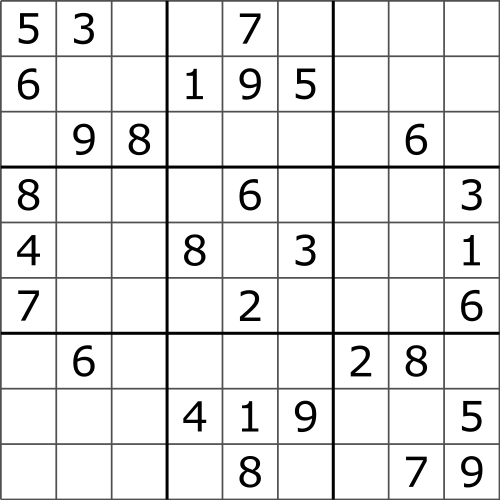
\includegraphics[width=150pt]{pic1.png}
	\hspace{30pt}
	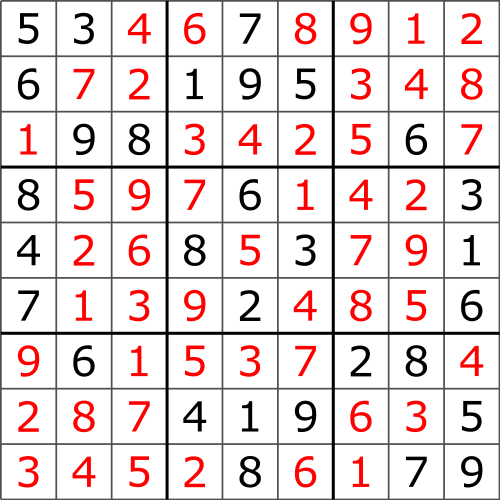
\includegraphics[width=150pt]{pic2.png}
	\caption{Example of a Normal Sudoku Puzzle and its Solution}
\end{figure}

In this project we want to design an AI engine to play Sudoku game. The Sudoku will not only be the classic $ 9\times9 $ playing board, but also bigger size Sudoku and Sudoku with irregular cells, by introducing new algorithms. Figure \ref{FIg:IrregSudoku} provides an example of an irregular Sudoku Puzzle.
\begin{figure}[h]
	\label{FIg:IrregSudoku}
	\centering
	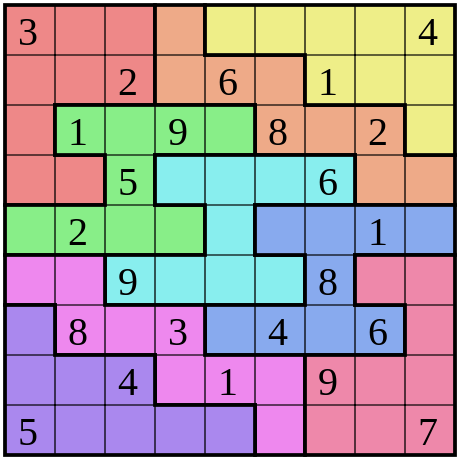
\includegraphics[width=150pt]{pic3.png}
	\hspace{30pt}
	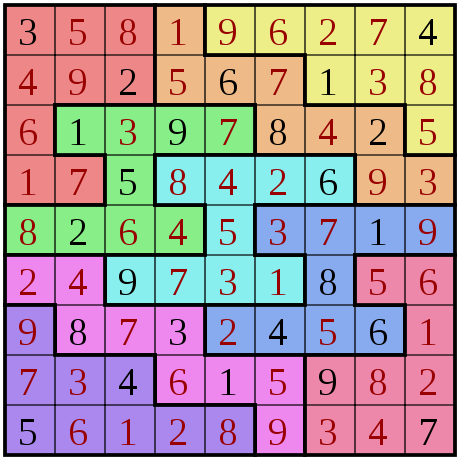
\includegraphics[width=150pt]{pic4.png}
	\caption{Example of an Irregular Sudoku Puzzle and its Solution}
\end{figure}

\section{Infrastructure}
First of all, to test the perfomance of Sudoku algorithms for normal $9\times 9$ Sudoku games, we run our proposed algorithm and the trivial trackback algorithm on the open $9\times 9$ Sudoku dataset \cite{}, which includes one million puzzles and each of them has exactly one solution.

Our algorithm also used for larger or irregular puzzles, but there are few corresponding open large dataset. Hence we wrote our own generater to generate irregular puzzles of arbitrary size and test the algorithms on these generated puzzles. However, it is hard to gurantee each generated puzzle has only one solutions when generating very large puzzles.

Here are multiple criterions that can be used to measure the performances of Sudoku algorithms, and we choose two simple criterions to compare our proposed algorithm with the already-known one:
\begin{enumerate}
	\item Average time consumed to solve one puzzle. Obviously this is an intuitive measure for performance and can reflect how well an algorithm works in practice. However, this criterion also depends on how to implemente the algorithm and which machine the program is running on.
	\item The number of node explored in the search procedure. This criterion is independent of specific implementation and could reflect goodness of our heuristic function. But this measure ignores the cost of calculating heuristic function, so that an aggressive heuristic that explores less nodes may cost much more time in practice.
\end{enumerate}

\section{Literature review}

Various algorithms have been implemented to solve the Sudoku problem \cite{sspr}. A logic-based algorithm, mimicking the way a human would solve the puzzle, is adequate to attain a solution. Harder puzzles, where guessing is required, can be solved using backtracking algorithms \cite{sspr}. The problem with back tracking is that the efficiency of the algorithm is dependent on the number of guesses required to solve the puzzle \cite{tj}. A solution to this problem could lie in using stochastic optimization techniques.

Some work has been done on solving Sudoku using stochastic optimization techniques [2-4]. The primary motivation behind using these techniques is that difficult puzzles can be solved as efficiently as simple puzzles. This is due to the fact that the solution space is searched stochastically until a suitable solution is found \cite{tj}. Hence, the puzzle does not have to be logically solvable or easy for a solution to be reached efficiently.

Furthermore, stochastic optimization techniques are used to find the global optimum of a problem which contains many local optima \cite{aj}. Due to the constraint nature of Sudoku, it is very likely to find a solution which satisfies some of the constraints but not all of them, hence finding a local optimum. Due to the stochastic nature of these techniques, the solution space is still searched even though a local optimum has been found, allowing for the global optimum to be detected.

Another solution is to improve the exploration process so that we can find a feasible solution before expanding too much nodes. Therefore, a well-designed heuristic function is very important to our exploration process. A brute force algorithm visits the empty cells in some order, filling in digits sequentially, or backtracking when the number is found to be not valid \cite{bt}. Minimum Remaining Values ordering is proposed when faced with the decision on what order should its cells be explored \cite{rl}. However, when faced with which value should be tried first in a cell, most solvers just use lexicographical order to decide it. Similar to the order of cell exploration, Minimum Remaining Values ordering is also considered to work well in this choice \cite{rl}, but the definition of this heuristic is not very clear. This part can be improved a lot.

Some other work has been done on reducing Sudoku puzzle to graph coloring problems, or more often an exact cover problem. Then they want to use Knuth’s elegant Dancing Links algorithm (DLX) \cite{dlx}. However, this technique is not very direct to the origin puzzle and the efficiency is restricted by the DLX algorithm. Thus, we do not consider this algorithm.


\section{Algorithm Description}

The input of a Sudoku game is a digit sequence with totally 81 digits, each of which represents the given number in the puzzle, from left to right, top to bottom. We will use $ 0 $ to represent the empty grids to be fill out. And the expected solution, the output, is also a 81-digit sequence, which is the right digit assignment satisfying the rules. There is no $ 0 $ in the output.

We are going to develop some new algorithms to speed up the solving process. Based on back tracing algorithm, we assign the nonempty position's value to the initial dictionary variable, which is the table of our playing board. When we meet $ 0 $, assign the list $ [1,2,3,4,5,6,7,8,9] $ to the entry. Then eliminate the digits in each grid which violate the constraint rules in current state. If a grid's list remains only one digit, assign it the grid and update the current state. Naked Twin or Triplets trick, which is also called Naked Twin exclusion rule, is used,  in order to speed up this process. Even if the pair of grids are not assigned, we can also use these naked twins (or triplets) to eliminate some candidates. Implement recursion techniques to create depth-first-search trees for solving hard sudokus that need guess work in any particular box to proceed. If we can find a feasible solution, just halt and return this solution.


\section{Advanced Variation}
In the search process we need guess the number in every blank box to proceed. Here the right choice, or reasonable attempt priority is very important to our solver, which can help us find a feasible solution much faster. Therefore, a reasonable and novel heuristic function, instead of simple natural number order, is a very good tool to decide the order of trial. For now we use a specially designed heuristic function to speed up our search. Basically, this heuristic function is calculated by summing over the number of possible values in each cell and then minus the number of cells. It is easy to see that a valid solution is reached if and only if the heuristics function is exactly zero.  The intuition behind the defintion of heuristics function is that when the function value is a small non-negative integer then the further search procedure from this state would be relatively quick since the braches in search tree from that state would be rather sparse. However, sometimes there may be no valid number that can be put into some cell. In this case we let the heuristics function be infinity.

Moreover, we will also try to solve Sudoku with bigger size. The advantage of implementing heuristic function will be more significant with the growth of the size. We will also try to solve for Sudoku with irregular cells. The performance of the new algorithm can be measured by the time it consumes to solve the testing set problems, compared to that consumed by the simple back tracing solver. This evaluation also involves the design of larger Sudoku, since this data set is hard to find on the Internet.

\section{Experiment Results}
Now we have completed the basic back tracing algorithm (which can be seen in util.py). We can run the python file and type the input ($n^2$ numbers for normal $n\times n$ Sudoku Puzzle where $n$ is a complete square number), and then we can get one of its solotions. This algorithm will also use some other novel tricks, and will be generalized to a more universal solver so that we can solve the Sudoku Puzzle with irregular blocks.

\vspace{2.5ex}
\noindent
\includegraphics[height=6.5cm]{example}
%%%%%%%%%%%%%%%%%%%%%%%%%%%%%%%%%%%%%%%%%%%%%%%%%%%%%%%%%%%%%
% Begin edit from here

% End edit to here
%%%%%%%%%%%%%%%%%%%%%%%%%%%%%%%%%%%%%%%%%%%%%%%%%%%%%%%%%%%%%
\begin{thebibliography}{}
	\bibitem[1]{sspr} G. Santos-García and M. Palomino. Solving Sudoku Puzzles with Rewriting Rules. Electronic Notes in Theoretical Computer Science, 17(4), 79-93.
	\bibitem[2]{tj}T. Mantere and J. Koljonen. Solving and Rating Sudoku Puzzles using Genetic Algorithms. Proceeding of the IEEE Congress on Evolutionary Computation, 1382-1389.
	\bibitem[3]{rl}R. Lewis. Metaheuristics can Solve Sudoku Puzzles. Journal of Heuristics Archive, 13(4), 387-401.
	\bibitem[4]{aj}A. Moraglio and J. Togelius. Geometric Particle Swarm Optimization for Sudoku Puzzles. Webpage: http://julian.togelius.com/Moraglio2007Geometric.pdf.
	\bibitem[5]{dlx}Knuth, Donald. "Dancing links". Millennial Perspectives in Computer Science. P159. 187. arXiv:cs/0011047 Freely accessible.
	\bibitem[6]{bt}Norvig, Peter. "Solving Every Sudoku Puzzle". Peter Norvig (personal website). Archived from the original on 20 Oct 2016.
\end{thebibliography}

\end{spacing}
\end{document}

%%%%%%%%%%%%%%%%%%%%%%%%%%%%%%%%%%%%%%%%%%%%%%%%%%%%%%%%%%%%%
